% Author: Joseph Rowell

% Version: 3.0
% This work is licensed under a Creative Commons Attribution 4.0 International License. Please acknowledge accordingly.

% VISIT https://imagestore.ucl.ac.uk/ FOR UCL BANNERS OF DIFFERENT SUBJECT COLOURS
% Change \YourName command in Packages 
\documentclass[12pt, a4paper]{report}
\usepackage[T1]{fontenc}
\usepackage[latin1]{inputenc}
\usepackage[english]{babel}
\usepackage{siunitx}
\usepackage{graphicx}
\usepackage{tipa} % for the \ark{} command
\usepackage{graphics} % for pdf, bitmapped graphics files
%\usepackage{times} % assumes new font selection scheme installed
\usepackage{amsmath}
\usepackage{latexsym}
\usepackage{amscd}% for commutative diagrams
\usepackage{mathrsfs} %this package is for the script font \mathscr
\usepackage{relsize}
\usepackage{delarray}

\usepackage{datatool}% SOrted list http://ctan.org/pkg/datatool

\usepackage[nottoc]{tocbibind} % Adds bibliography to TOC
%Also adds roman numeral pages to TOC

\usepackage{glossaries}

\usepackage{pstricks}
\usepackage{theorem}
\usepackage{changepage}
\usepackage{euscript}
\usepackage{textcomp}
\usepackage{esvect}
\usepackage{parskip}
\usepackage{placeins}
\usepackage{subfigure}
% \usepackage{subcaption}
\usepackage{array}
\usepackage{delarray}
\usepackage{stmaryrd}
\usepackage{fancyhdr}
\usepackage{graphpap}
\usepackage{makeidx}
\usepackage{enumerate}
\usepackage{esint}
\usepackage{datetime}
\usepackage{caption}
\usepackage{smartdiagram}
\usesmartdiagramlibrary{additions}
%Set Abstract Page
\usepackage{abstract}
\setlength{\absleftindent}{-5mm}
\setlength{\absrightindent}{-5mm}

%Colour definitions - put before TikZ
\usepackage{color}
\definecolor{igreen}{rgb}{0.0, 0.56, 0.0}
\usepackage{xcolor, colortbl}
\colorlet{gred}{-red!75!green!65!}
\colorlet{mamber}{-red!75!green!15!blue!50!}
\colorlet{grown}{-red!75!blue!20!green}
\colorlet{bled}{-red!85!blue!40!green!45!}
\colorlet{waters}{cyan!25} % Define color for the water
\colorlet{water}{cyan!25!green!20!} % Define color for the water
\definecolor{grin}{HTML}{00F9DE}
\usepackage{rotating}
\providecommand{\keywords}[1]{\textbf{\textit{Keywords---}} #1}

% For faint dotted table line
\usepackage{arydshln}
\setlength{\dashlinedash}{.4pt}
\setlength{\dashlinegap}{.8pt}

\usepackage{booktabs}
\usepackage{graphicx}
\usepackage{tikz}
\usepackage{tikz-3dplot}
\usetikzlibrary{
arrows,
arrows.meta,
automata,
backgrounds,
calc,
decorations,
decorations.pathmorphing,
decorations.pathreplacing,
decorations.fractals,
external,
fit,
matrix,
petri,
positioning,
shadows,
shapes,
shapes.multipart,
topaths,
intersections
}
\usepackage{eso-pic}
\def\ba{\begin{array}}
\def\ea{\end{array}}
\def\beann{\begin{eqnarray*}}
\def\eeann{\end{eqnarray*}}
\def\bea{\begin{eqnarray}}
\def\eea{\end{eqnarray}}
\def\bsy{\boldsymbol}
\def\gray#1{{\color{gray}#1}}

%% COUNTERS
\setcounter{MaxMatrixCols}{20}
\renewcommand{\thesection}{\arabic{section}}
\renewcommand{\thesection}{\thechapter.\number\numexpr\value{section}}
\renewcommand{\thesubsection}{\thesection.\number\numexpr\value{subsection}}
%%For changemargin
\def\quote{\list{}{\rightmargin\leftmargin}\item[]}
\let\endquote=\endlist 
\def\changemargin#1#2{\list{}{\rightmargin#2\leftmargin#1}\item[]}
\let\endchangemargin=\endlist 
\makeatletter
\newlength\qvec@height
\newlength\qvec@depth
\newlength\qvec@width
\newcommand{\qvec}[2][]{
    \settoheight{\qvec@height}{$#2$}
    \settodepth{\qvec@depth}{$#2$}
    \settowidth{\qvec@width}{$#2$}
  \def\qvec@arg{#1}
  \raisebox{.2ex}{\raisebox{\qvec@height}{\rlap{% 
    \kern.05em
    \begin{tikzpicture}[scale=1,shorten >=-3pt,shorten <=-3pt]
    \pgfsetroundcap
    \coordinate (Stx) at (.05em,0) ;
		\coordinate (Arx) at (\qvec@width-.05em,0) ;
    \draw[->](Stx) to[bend left] (Arx);
    \end{tikzpicture}
  }}}
  #2
}
\makeatother
\makeatletter
\newlength\pvec@height
\newlength\pvec@depth
\newlength\pvec@width
\newcommand{\pvec}[2][]{
    \settoheight{\pvec@height}{$#2$}
    \settodepth{\pvec@depth}{$#2$}
    \settowidth{\pvec@width}{$#2$}
  \def\pvec@arg{#1}
  \raisebox{.2ex}{\raisebox{\pvec@height}{\rlap{% 
    \kern.05em
    \begin{tikzpicture}[scale=1,shorten >=-3pt,shorten <=-3pt]
    \pgfsetroundcap
    \coordinate (Stx) at (.05em,0) ;
		\coordinate (Arx) at (\pvec@width-.05em,0) ;
    \draw[->](Stx) to[bend right] (Arx);
    \end{tikzpicture}
  }}}
  #2
}
\makeatother
\makeatletter
\newlength\vvec@height%
\newlength\vvec@depth%
\newlength\vvec@width%
\newcommand{\vvec}[2][]{%
  \ifmmode%
    \settoheight{\vvec@height}{$#2$}%
    \settodepth{\vvec@depth}{$#2$}%
    \settowidth{\vvec@width}{$#2$}%
  \else 
    \settoheight{\vvec@height}{#2}%
    \settodepth{\vvec@depth}{#2}%
    \settowidth{\vvec@width}{#2}%
  \fi%
  \def\vvec@arg{#1}%
  \def\vvec@dd{:}%
  \def\vvec@d{.}%
  \raisebox{.2ex}{\raisebox{\vvec@height}{\rlap{%
    \kern.05em%
    \begin{tikzpicture}[scale=1]
    \pgfsetroundcap
    \draw (.05em,0)--(\vvec@width-.05em,0);
    \draw (\vvec@width-.05em,0)--(\vvec@width-.15em, .075em);
    \draw (\vvec@width-.05em,0)--(\vvec@width-.15em,-.075em);
    \ifx\vvec@arg\vvec@d%
      \fill(\vvec@width*.45,.5ex) circle (.5pt);%
    \else\ifx\vvec@arg\vvec@dd%
      \fill(\vvec@width*.30,.5ex) circle (.5pt);%
      \fill(\vvec@width*.65,.5ex) circle (.5pt);%
    \fi\fi%
    \end{tikzpicture}%
  }}}%
  #2%
}
\makeatother
\def\ba{\begin{array}}
\def\ea{\end{array}}
\def\beann{\begin{eqnarray*}}
\def\eeann{\end{eqnarray*}}
\def\bea{\begin{eqnarray}}
\def\eea{\end{eqnarray}}
\def\bsy{\boldsymbol}
\def\gray#1{{\color{gray}#1}}
\usepackage{titlesec}
\usepackage{multirow}
%To reference within text
\usepackage{hyperref}
%\usepackage{ieeetr}
\usepackage{lipsum}
\usepackage{tikz-cd}
\usepackage{float}
\usepackage{titling}
\usepackage{epigraph}
\usepackage[title, titletoc]{appendix}
\setlength\epigraphwidth{8cm}
\setlength\epigraphrule{0pt}

\titleformat{\chapter}{\normalfont\LARGE}{\thechapter\,$\vert$}{20pt}{\LARGE}{\setcounter{chapter}{0}}
\setlength{\headheight}{15pt}
\titlespacing*{\chapter}{0pt}{-70pt}{40pt} %Move chapter titles up
% Title page logos:
\makeatletter
\newcommand\BackgroundPicturea[3]{
	\setlength{\unitlength}{1pt}
	\put(0,\strip@pt\paperheight){
		\parbox[t]{\paperwidth}{
			\vspace{#2}\hspace{#3}
			\mbox{\includegraphics[scale=0.5]{#1}}
}}}
\newcommand\BackgroundPictureb[3]{
	\setlength{\unitlength}{1pt}
	\put(0,\strip@pt\paperheight){
		\parbox[t]{\paperwidth}{
			\vspace{#2}\hspace{#3}
			\mbox{\includegraphics[scale=0.3]{#1}}
}}}
\makeatother
% For my abbreviations
\newcommand{\abbrlabel}[1]{\makebox[3cm][l]{\textbf{#1}\ \dotfill}}
\newenvironment{abbreviations}{\begin{list}{}{\renewcommand{\makelabel}{\abbrlabel}}}{\end{list}}
% Line Spacing%%%%%%%%%%%%%%%%%%%%%%%%%%%%%%%%%
\usepackage{setspace}
\setstretch{1.5}
%Set of command is for the changemargin environment
\def\quote{\list{}{\rightmargin\leftmargin}\item[]}
\let\endquote=\endlist 
\def\changemargin#1#2{\list{}{\rightmargin#2\leftmargin#1}\item[]}
\let\endchangemargin=\endlist
%Replace Contents to Table of Contents	
\addto\captionsenglish{
	\renewcommand{\contentsname}%
	{Table of Contents}
	\setcounter{tocdepth}{3}% Include \subsubsection in ToC
	\setcounter{secnumdepth}{3}% Number \subsubsection in ToC
	}
\renewcommand{\listfigurename}{List of Figures}
\renewcommand{\listtablename}{List of Tables}


\usepackage{xcolor}
\usepackage{listings}
\usepackage{xcolor}

%New colors defined below
\definecolor{codegreen}{rgb}{0,0.6,0}
\definecolor{codegray}{rgb}{0.5,0.5,0.5}
\definecolor{codepurple}{rgb}{0.58,0,0.82}
\definecolor{backcolour}{rgb}{0.95,0.95,0.92}

%Code listing style named "mystyle"
\lstdefinestyle{mystyle}{
  backgroundcolor=\color{backcolour}, commentstyle=\color{codegreen},
  keywordstyle=\color{magenta},
  numberstyle=\tiny\color{codegray},
  stringstyle=\color{codepurple},
  basicstyle=\ttfamily\footnotesize,
  breakatwhitespace=false,         
  breaklines=true,                 
  captionpos=b,                    
  keepspaces=true,                 
  numbers=left,                    
  numbersep=5pt,                  
  showspaces=false,                
  showstringspaces=false,
  showtabs=false,                  
  tabsize=2
}

%"mystyle" code listing set
\lstset{style=mystyle}
\lstset{basicstyle=\tiny,style=mystyle} 

\renewcommand\lstlistingname{Listing}
\renewcommand\lstlistlistingname{Listings}
\def\lstlistingautorefname{Alg.}

\newcommand{\R}{\mathbb{R}}
\newcommand{\U}{\mathbb{U}}
\newcommand{\YourName}{Your Name}

% Algorithms and pseudocode packages
\usepackage{algorithm}
\usepackage{algpseudocode}
\hypersetup{pdftitle = Project Report, pdfauthor = {First Last}, pdfstartview=FitH, pdfkeywords = essay, pdfpagemode = FullScreen, colorlinks, anchorcolor = black, citecolor = blue, urlcolor=blue, filecolor=green, linkcolor = black, plainpages = false}
%%%%%%%%%%%%%%%%%%%%%%%%%%%%%%%%%%%%%%%%%%%%%%%%%%%%%%%%%%%%%%%%%%%%%%%
\pagestyle{fancy}
\rhead{}
\chead{}
\lhead{University College London}
\lfoot{\date{}}
\cfoot{}
\rfoot{\thepage}
% Top and Bottom Line Rules

\renewcommand{\headrulewidth}{0.4pt} %0.4pt
\renewcommand{\footrulewidth}{0.4pt}
\fancyheadoffset{8pt}
\fancyfootoffset{8pt}
% Line spacing
\renewcommand{\baselinestretch}{1.5} %1.5
%%%%%%%%%%%%%%%%%%%%%%%%%%%%%%%%%%%%%%%%%%%%%%%%%%%%%%%%%%%%%%%%%%%%%%%
\makeglossaries

\newglossaryentry{latex}
{
    name=latex,
    description={Is a markup language specially suited 
    for scientific documents, this term is printed in conclusion }
}

%Sorted list
\newcommand{\sortitem}[1]{%
  \DTLnewrow{list}% Create a new entry
  \DTLnewdbentry{list}{description}{#1}% Add entry as description
}
\newenvironment{sortedlist}{%
  \DTLifdbexists{list}{\DTLcleardb{list}}{\DTLnewdb{list}}% Create new/discard old list
}{%
  \DTLsort{description}{list}% Sort list
  \begin{itemize}%
    \DTLforeach*{list}{\theDesc=description}{%
      \item \theDesc}% Print each item
  \end{itemize}%
}
\date{}

\title{Interesting Scientific Title}
\author{\\ \Large{\YourName}
\\ Supervisors: Supervisor Name
\\ Faculty of Engineering
\\ Department of Computer Science
\\ 
\\
\\ University College London
\\
A Project Report Presented in Partial Fulfillment of the Degree \\ \textit{MSc Your Degree}
\\ \\
September 2022
}
%%%%%%%%%%%%%%%%%%%%%%%%%%%%%%%%%%%%%%%%%%%%%%%%%%%%%%%%%%%%%%%%%%%%%%%
\begin{document}
%Adjust logo positions here
% \AddToShipoutPicture*{\parbox[t][\paperheight][t]{\paperwidth}{%
%           \includegraphics[width=\paperwidth]{\BackgroundPicturea{Logos/ucl_long%_logo.png}{3in}{3in}}
%           }}
% \AddToShipoutPicture*{\centering\BackgroundPictureb{Logos/Bentham2011_065_c623d.jpg}{3in}{3.7in}}
\AddToShipoutPictureBG*{%
  \AtPageUpperLeft{%
    \raisebox{-\height}{%
      \includegraphics[width=\paperwidth]{Logos/UCL_page_header.png}% Change this to no_dept if not Compsci
    }}
}
\AddToShipoutPicture*{%
      \parbox[t][\paperheight][t]{\paperwidth}{%
          \includegraphics[width=\paperwidth]{Logos/UCL_page_footer.png}
      }}
      

\thispagestyle{headings}
\maketitle
\FloatBarrier
\pagenumbering{roman}

\newpage
\thispagestyle{empty}
\begin{center}
I dedicate this ...
\end{center}

\newpage
\thispagestyle{empty}
\vspace*{\fill}
\begin{center}
Copyright \copyright  \thinspace 2022 by \YourName \\ All Rights Reserved
\end{center}
\vspace*{\fill}
\newpage
\thispagestyle{empty}
%\epigraph{The Book of Nature is written in the language of mathematics.}{--- \textup{Galileo Galilei}}
\epigraph{The computer was born to solve problems that did not exist before.}{--- \textup{Bill Gates}}

\thispagestyle{empty}
\chapter*{Acknowledgements}
I would like to express ...


\thispagestyle{empty}
\chapter*{Declaration}
I, \YourName,  I declare that the thesis has been composed by myself and that the work has not be submitted for any other degree or professional qualification. I confirm that the work submitted is my own, except where work which has formed part of jointly-authored publications has been included and referenced. \\
% \begin{figure}[H]
% \includegraphics{Logos/signature.PNG}
% \end{figure}
% \vspace{-2cm}
\noindent\begin{tabular}{ll}
 & 01/01/22 \\
\makebox[2.5in]{\hrulefill} & \makebox[2.5in]{\hrulefill}\\
\textit{Signature} & \textit{Date}\\
\end{tabular}

\thispagestyle{empty}
\begin{abstract}
\lipsum[1-2]

\keywords{Keyword1 - Keyword2 - Keyword3}
% \vspace{-10mm} %To remove added white space after
\end{abstract}

\tableofcontents

\thispagestyle{plain}
\listoffigures
\listoftables
\lstlistoflistings
\chapter*{List of Abbreviations}
%\begin{abbreviations}
%sort alphabetically 
\begin{sortedlist}
  \sortitem{CNN:     Convolutional Neural Network}
  \sortitem{SLAM:    Simultaneous Localization And Mapping}
  \sortitem{GNSS:    Global Navigation Satellite System}
  \sortitem{KF:      Kalman Filter}
  \sortitem{MAP:     Maximum a Posteriori}
  \sortitem{ML:      Maximum Likelyhood}
  \sortitem{IMU:     Inertial Measurement Unit}
  \sortitem{UAV:     Unmanned Aerial Vehicle}
  \sortitem{EKF:     Extended Kalman Filter}
  \sortitem{GPS:     Global Positioning System}
  \sortitem{SKLearn: SciKitLearn}
  \sortitem{BA:      Bundle Adjustment}
  \sortitem{ATE:     Absolute Trajectory Error}
  \sortitem{RPE:     Relative Pose Error}
  \sortitem{VO:      Visual Odometry}
  \sortitem{VSLAM:   Visual Simultaneous Localisation and Mapping}
  \sortitem{SfM:     Structure From Motion}
 \end{sortedlist}
%\end{abbreviations}
\chapter{Project Plan}
\label{Chap1}
\section{Problem}
\section{State-of-the-art}
\section{Aims and Objectives}
\section{Work Plan}
\section{Deliverables}
\section{Evaluation}
\section{Project Timeline}
%gantt
\begin{figure}[ht]% h for here
\centering
\includegraphics[width=1\textwidth]{Figures/gantt_example.PNG}
\end{figure}
\chapter{Introduction and Background}
\label{Chap2}
\pagenumbering{arabic}
\section{Motivation}
\lipsum[1-3]
\section{Aims}
\lipsum[6]
\section{Thesis Outline}
The remainder of this report is organised as follows:
\begin{itemize}
    \item[] \textbf{Chapter} \hyperref[Chap2]{\textbf{2}} --- Introduces the related work and literature review performed in preparation for this project.
    \item[] \textbf{Chapter} \hyperref[Chap3]{\textbf{3}} --- Introduces the methodology used in creating the feature distinction algorithm, including technical challenges encountered.
    \item[] \textbf{Chapter} \hyperref[Chap4]{\textbf{4}} --- Introduces the Results and Analysis of the performed method.
    \item[] \textbf{Chapter} \hyperref[Chap5]{\textbf{5}} --- Introduces the discussion of the results and possible future work.
    \item[] \textbf{Chapter} \hyperref[Chap6]{\textbf{6}} --- Concludes and reflects on the project and its outcomes overall.
\end{itemize}
\section{Related Work}

\chapter{Methodology}
\label{Chap3}
We can cite an article as an example \cite{DeepMindRef}. \lipsum[4-8]
\begin{table}[H]
   \caption{Example Table }\label{tab:exampleTable}
   \small
   \centering
   \begin{tabular}{lccccr}
   \toprule[\heavyrulewidth]\toprule[\heavyrulewidth]
   \textbf{C1} & \textbf{C2} & \textbf{C3} & \textbf{C4}\\ 
   \midrule
\multirow{3}{*}{\textbf{Row}}& Val & Val & \textcolor{igreen}{GreenVal}\\
   & & Val  & \textcolor{igreen}{Val}\\
& &  & \textcolor{igreen}{Example}\\ \hdashline
   \bottomrule[\heavyrulewidth] 
   \end{tabular}
\end{table}


% Example Algorithm and pseudocode
\begin{algorithm}
\caption{An algorithm with caption}\label{alg:cap}
\begin{algorithmic}
\Require $n \geq 0$
\Ensure $y = x^n$
\State $y \gets 1$
\State $X \gets x$
\State $N \gets n$
\While{$N \neq 0$}
\If{$N$ is even}
    \State $X \gets X \times X$
    \State $N \gets \frac{N}{2}$  \Comment{This is a comment}
\ElsIf{$N$ is odd}
    \State $y \gets y \times X$
    \State $N \gets N - 1$
\EndIf
\EndWhile
\end{algorithmic}
\end{algorithm}

%Ensure to put system information, perhaps appendix
%section{System Information}
\chapter{Results and Analysis}
\label{Chap4}
\lipsum[1-4]
\begin{figure}
    \centering
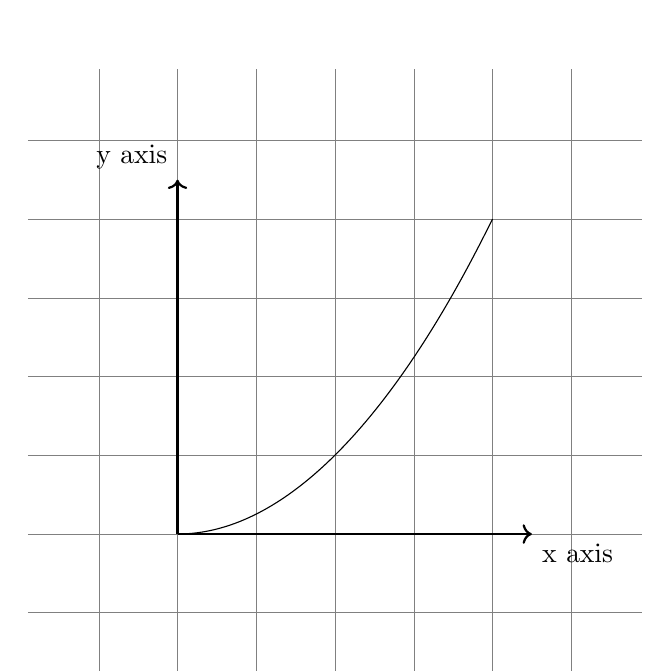
\begin{tikzpicture}
    \draw[step=1cm,gray,very thin] (-1.9,-1.9) grid (5.9,5.9);
    \draw[thick,->] (0,0) -- (4.5,0) node[anchor=north west] {x axis};
    \draw[thick,->] (0,0) -- (0,4.5) node[anchor=south east] {y axis};
    \draw (0,0) parabola (4,4);
\end{tikzpicture}
\caption{Example TikZ Figure}
\end{figure}
\chapter{Discussion}
\label{Chap5}
\lipsum[9-10]
\footnote{Only now do I understand latex footnotes}

\chapter{Conclusion}
\label{Chap6}
\Gls{latex} 
\renewcommand{\bibname}{References}
\bibliographystyle{ieeetr}
\bibliography{Bibliography.bib}

% APPENDIX
\begin{appendices}
\chapter{Appendix}
\begin{lstlisting}[language = Matlab, caption= Listing Example]
%Put code here
\end{lstlisting}
\end{appendices}

% GLOSSARY
\clearpage
\printglossaries

% INDEX?

\end{document}